\documentclass{iuphd_proposal}
\usepackage[utf8]{inputenc}
\usepackage{cite}

% exta packages
\usepackage{graphicx, caption, subfig, setspace, soul, color, paralist}
% \usepackage{subcaption}

\usepackage{rotating}
\usepackage{relsize}
\usepackage{booktabs}
\usepackage{tikz}
\usepackage{multirow}
\usepackage{adjustbox}
\usepackage{array}
\usetikzlibrary{arrows,shapes}

% extra commands
%\captionsetup[figure]{font={stretch=1.1}}
\newcommand{\fixme}[1]{\sethlcolor{yellow}\hl{#1}}
\newcommand{\xhdr}[1]{\vspace{4pt}\noindent {\textit{\textbf{#1.}}}}
%\newcommand{\rebuttal}[1]{\textcolor{red}{#1}}
\newcommand{\rebuttal}[1]{#1}


%data for Title Page
\title{Web-scale Visual Content Mining with Computer Vision Methods}
\author{}
\date{}

%data for Acceptance Page
\committeechair{}
\readertwo{}
\readerthree{}
\readerfour{}
\defensedate{}


%data for Copyright Page
\cryear{}

\begin{document}
\maketitle

% \acceptancepage

% \copyrightpage

%\begin{dedication}
%\end{dedication}

% \begin{acknowledgments}
% \end{acknowledgments}

%\begin{preface}
%\end{preface}

\begin{abstract}
Social media provides low-cost and easy access to a large number of images with a wide variety of visual content. With this new source of large-scale image data, there is a critical demand for novel, scalable methods that can understand the information behind the visual content. For example, photos shared on social media are usually accompanied with temporal and location metadata, user profiles and textual annotations. When we integrate the visual content by user profiles or location tags, we can estimate a large variety of information. For example, we can help research in Psychology when we are interested in the human beings who take these photos and in Ecology when we are interested in the natural scenes as the visual content. 
These attractive properties of this new data source also bring us new challenges.
Being able to efficiently processing data with advanced computer vision techniques is an important requirement.
To accommodate the graphical structure of metadata in social media, we also need to develop new models and systems.

This thesis introduces three projects: a cloud based robotic system testing the feasibility of a memory and computing consuming task to work in near real time; a data mining application supporting Psychology research in gender differences in preference of color; and a natural event tracking system on a continental scale.
We design and implement a cloud based system to apply these algorithms for object detection and recognition with the best precision in near real time. We test our method on an aerial autonomous vehicle.
We take advantage of this new data source for psychology research. Based on the color pixels of these photos, we analyze the gender difference in color preference. We study the distribution of color pixels with respect to genders of photographers across geographic locations and content. We find strong sex differences for the predominant reddish and bluish hues, with female users uploading more photographs containing more reddish pixels and male users uploading more photographs containing more bluish pixels.  Furthermore, we take Google Street View to represent the color distribution in the environment, and compare with Flickr photos in three popular outdoor locations. We observe the overall preference of saturated color and reddish color of human compared to the environment.
By mining visual content on social media websites web-scale images further benefit studies about the state of nature. We develop and evaluate three models to study ecology phenomena such as snow and vegetation coverage.
First, we learn a binomial distribution to model the probability of the appearance of a natural phenomenon. 
Then, we compute the histogram of the confidence of each image being a positive evidence. Based on this histogram, we learn a classification model for the confidence of each user, and similarly apply this method to predict for each time and location.
Finally, inspired by the study of multiple instance learning, we propose an end to end system taking a sequence of images as input and giving predictions as the final output of this holistic system. This process will happen twice, once for users and once for each day and location. The two aggregating processes are optimized simultaneously.

\end{abstract}

\tableofcontents

\chapter{Introduction}
Social media encourages the development of online social network, connecting billions of users sharing status and comments in text and multimedia format.
These increasingly large number of multimedia files such as photographs become a new source of web-scale data with high variety and publicly available.
Along with the image files and text annotations, social networking websites and mobile applications also record user profiles as well as time and location metadata of users activity.
This new data source is quite noisy but is also easy accessible. 
It collects data constantly from a broad selection of locations on this earth. 
To better understand the information behind this large collection of data, there is a critical demand for novel, scalable methods to navigate the visual content together with the textual annotation and user activity.
Researchers from computer vision, multimedia, data mining and machine learning become more and more interested in this interdisciplinary area, especially with the progress in computer vision and with the development of computing capacity.

When we integrate the visual content by the metadata of user activities, we will provide a very low-cost, large scale data source for researchers in many areas of social and natural science.
For example, we will help research in social science when we are interested in the human behavior of those who take photos and share on social media, and in nature science when we are interested in the natural scenes and the associated location, time and user profile.
These attractive properties of this new data source also bring us new challenges. 
Being able to efficiently processing data with advanced computer vision techniques is an important requirement.
To accommodate the graphical structure of metadata in social media, we also need to develop new models and systems.
% challenge of color project

This thesis presents our works of solving problems in three aspects to facilitate research in different areas with web-scale image data.


\begin{compactitem}[--]
        \item In \textbf{Chapter 2} we design and implement a cloud based system to apply these algorithms for object detection and recognition with the best precision in near real time. We test our method on an aerial autonomous vehicle.
	\item In \textbf{Chapter 3} we take advantage of this new data source for psychology research. Based on the color pixels of these photos, we analyze the gender difference in color preference. We study the distribution of color pixels with respect to genders of photographers across geographic locations and content. We find strong sex differences for the predominant reddish and bluish hues, with female users uploading more photographs containing more reddish pixels and male users uploading more photographs containing more bluish pixels.  Furthermore, we take Google Street View to represent the color distribution in the environment, and compare with Flickr photos in three popular outdoor locations. We observe the overall preference of saturated color and reddish color of human compared to the environment.
	\item In \textbf{Chapter 4} we present an example of web-scale images further benefit studies about the state of nature. We develop and evaluate three models to study ecology phenomena such as snow and vegetation coverage.
First, we learn a binomial distribution to model the probability of the appearance of a natural phenomenon based on the number of users uploading images with and without the target phenomenon. 
Then, we compute the histogram of the confidence of each image being a positive evidence. Based on this histogram, we learn a classification model for the confidence of each user, and similarly apply this method to build a histogram of user confidence in order to predict for each time and location.
Finally, inspired by the study of multiple instance learning, we propose an end to end system taking a sequence of images as input and giving predictions as the final output of this holistic system. For the main challenge of multiple instance learning, we use a network to aggregate a bag of evidence. This process will happen twice, once for users and once for each day and location. The two aggregating processes are optimized simultaneously.
\end{compactitem}



\chapter{Real-time, Cloud-based Ojbect Detection for Unmanned Aerial Vehicles}
\section{Introduction}
Web-scale visual data provides massive amount of information while requiring more complex models to take this advantage, therefore, whether we can apply computer vision techniques efficiently enough becomes a bottleneck question.
Robotics is a typical area in need of near real-time performance. Unmanned Aerial Vehicles (UAVs), as a type of the autonomous robotics systems, are increasingly intereting to researchers in recent years. 
They are widely used in applications including reconnaissance and surveillance, search-and-resuce, and infrastructure inspection.
%cite
Visual object detection is an important component of such UAV applications.
Moreover, it's also very challenging because of noisy image quality with complex scene and most importantly, the conflict of the near real-time performance requirement and the relatively long running time of advanced object recognition techniques.
Solving this problem not only improves the computer vision component on robotics systems, but also extend the object recognition models based on very large dataset to near real-time applications.

Object recognition performance is rapidly improving mostly based on Deep Learning techniques with Convolutional Neural Networks.
%cite
These deep models are trained with very large datasets and are typically consist of millions or billions of paramenters. These computational demanding techniques require the support of hardware including gigabytes of memory and high-end Graphics Processing Units (GPUs). Eventhough, the techniques with best accuracy are still far away from near real-time. According to these computation demand and running time problems, it's infeasible to apply these deep models to drones featuring low-cost and light-weight.
%cloud
Numerous studies have explored the benefits of ``Cloud Robotics''.
%cite
Cloud computing allows on-demand access to nearly unlimited computational resources, which is especially useful for customized hardware combination and periodical requirement of huge amounts of computation. In this project, we build our Deep Learning facilitated cloud system to fulfill the hardware requirement and solve the efficiency problem. In fact, because of the unpredictable network delay due to the communication with a remote cloud, we build a hybrid system especially with onboard processing for critical tasks requiring immediate reaction such as stability control. 

\section{Approach}
We use a Parrot AR.Drone 2.0 as a low-cost hardware platform
%cite{the navigation and control technology inside the ar. drone micro uav}
to test our cloud-based recognition system. It is small and lightweight, and can be operated both indoors and outdoors.
The AR.Drone 2.0 is equiped with two cameras. 
The bottom-facing camera with lower resolution of $320 \times 240$ while the front-facing camera has a higher resolution of $1280 \times 720$. 
To allow this drone to see objects on the ground, we mount a mirror at a $45^{\circ}$ angle to the front camera as in ~ref{fig:mirror}.

Our approach consists of four main components shown at top ~ref{fig:overview}. Each component is implemented as a node in the Robot Operating System (ROS), allowing it to communicate with others using the ROS transport protocol.
%~cite{ROS: an open-source robot operating system}
The controlling components and objectness estimation component are running on a laptop connected to the drone through the AR.Drone device driver package of ROS, over a WiFi link. On the other hand, the most computationally demanding component, the CNN based object detection node, runs on a remote cloud computing server that the laptop connects to via Internet.
The bottom of ~ref{fig:overview} shows the pipeline of image processing in our hybrid approach. 
The drone takes off and starts to search with the downward-facing camera. Given input video taken from this downward-facing camera, the objectness estimator node runs the BING algorithm to detect generic objects of every frame, and then takes a high resolution image with the front-facing camera if it detects candidate objects in the frame.
%~cite{Bing: Binarized normed gradients for objectness estimation at 300 fps}
Therefore, only the ``interested'' images that have a high likelihood to contain objects are sent to the cloud server, where the CNN based object detection node is running to recognize the target objects.

\section{Experimentsal Results}
We conducted three sets of experiments to demonstrate that our approach performs successfully in a realistic but controlled envrionment. 
In the first set of experiments, we focus on testing the accuracy of recent deep network based object detectors with aerial images taken by the drone.
Secondly, we evaluate the speed of our cloud based object detection approach, comparing with running time of the fastest deep learning based object detector on a local laptop. Finally, we verify our approach with the scenario of a drone searching for a target object in an indoor environment, as a simple simulation of a search-and-rescue or surveillance applicaiton. The first two sets of experiments were conducted on our aerial image dataset and the last experiment was conducted in an indoor room of about $3m \times 3m$.

\subsection{Object Detection Accuracy}
We first compared the ability of Faster R-CNNs with two recent state-of-the-art object detectors(YOLO
%cite{you only look once: unified..}
 and SSD
%cite{ssd:single shot multibox detector}
) to recognize aerial images taken by the drone.
YOLO and SSD are approaches that achieving real-time performance (faster than 30 FPS) on GPU by eliminating the most computationally demanding part(generating region proposals and computing CNN features for each region). 

%To make a fair comparison, we use models that are all pre-trained on the same dataset(Pascal VOC 2007 and Pascal VOC 2012). 
We collected 294 erial images of 20 object classes and annotated 578 objects in the images. These images have the same object classes as the Pascal VOC 2007 dataset and are collecte from two sources (some of them are taken by ourselves and the others are collected from 31 publicly available Youtube videos taken by the same drone as ours).
Table ~ref{tab:objdetection} shows average precision of each algorithm on htis dataset. Here the SSD300 model and SSD500 model have the same architecture and the only difference is the input image size($300 \times 300$ pixels vs. $500 \times 500$ pixels). YOLO and Fast YOLO also use similar architectures except Fast YOLO uses fewer convolutional layers (24 convolutional layers vs. 9 convolutional layers for Fast YOLO).

According to our experiment, Faster R-CNN achieved $83.9\%$ mean average precision (mAP) compared to YOLO models ($78.3\%$ and $79.4\%$) and two SSD models ($81.6\%$ and $82.6\%$).

\subsection{Recognition Speed on Cloud System}
Our second set of experiments evaluate the running time performance of the CNN-based object recognition testing the extent to which cloud computing could improve recognition times, and the variability of the unpredictable communication times. We use the same dataset as in the previous section and compare the speed of each algorithm using GPU on a simulated cloud machine.
We measure the running time including image loading, pre-processing, and output parsing (post-processing) time.

Fig. ~ref{fig:dot} shows the running time of each algorithm as a function of its accuracy. The result shows detection spped and accuracy are inverse related. Fast YOLO showed te highest speed (57.4 FPS) with the lowest accuracy (mAP $78.3\%$), while Faster R-CNN has the lowest speed (3.48 FPS) with the highest accuracy (mAP $83.9\%$).

Then we compare Fast YOLO on a local laptop versus Faster R-CNN on the simulated cloud. A comparison of these computing facilities are showed in Table ~ref{tab:hardware}. Fig. ~ref{fig:bar} shows the average running time of Fast YOLO on local machine is $7.31$ seconds per image while for Faster R-CNN running on remote cloud is $1.29$ seconds including latencies for sending each image to the cloud (which averaged about 600 ms) and for exchanging detected results and other command messages (which averaged 0.41 ms). Thus the cloud-based recognition performed about 5.7 times faster than the local Fast YOLO on average.

\subsection{Target Search with a Drone}
In the test senario, we use a screwdriver as a target object and scattered various distractor objects on the floor in the indoor test room. 
The drone started this object searching mission with lower-reolution downward-facing camera, and run the BING algorithm for finding generic objects given the input video.
When the drone finds any ``interesting'' objects on the floor, it switches to the front-facing camera to capture a photo at a higher resolution, then take picture of the candidate area and sends it to the cloud system ($t=3$s and $t=8$s).
After this, the drone switch the camera back to the downward-facing camera and proceeds to the other cadidate positions. The cloud system performs recognition in the meantime.
The drone performs the same steps until it finds a target object, at which point the mission is completed ($t=17$s).



\chapter{Assessing color preferences and sex differences using massive online data}
\section{Introduction}
Variation in human color preferences across cultures and sexes has not been well characterized. The majority of past studies have worked with relatively small samples of participants asked to make explicit decisions with limited stimuli consisting of blocks of single colors. 
Using this method, Hurlbert and Ling ~\cite{hurlbert2007biological} found a universal preference for bluish hues, along with a greater cross-cultural female preference for reddish hues.
They gave an evolutionary explanation related to the adaptive benefit to foraging females of seeking out a red object on a green background (e.g., fruit against leaves).  
Palmer and Schloss ~\cite{palmer2010ecological} argued that color preferences can be explained in terms of object preferences and associations between objects and colors, which can be influenced by evolution, culture, and individual experience.  The question of sex differences was left open in this paper.

We propose that large-scale novel data-mining of images available on the Web can overcome the limitation of study sizes. Moreover, the metadata associated with the web-scale images provides more interesting information for our complimentary studies.
When people upload their photos to social networks, they are sharing information about which scenes and types of photos they prefer.
By analyzing the color spectra over 15 million photographs on Flickr, an online photo-sharing network, we measure male and female preferences in an implicit (behavior-based) rather than explicit (ratings-based) manner and on a much larger scale than can be done in a lab experiment.
We find strong sex differences for the predominant reddish and bluish hues, with female users uploading more photographs containing more reddish pixels and male users uploading more photographs containing more bluish pixels.
To take a step towards exploring the reason for this difference and the relation of content preference and color preference, we analyze the least entropy textual tags used by photographers taking photos with most amount of color pixels in each hue interval. Furthermore, we take Google Street View to represent the color distribution in the environment, and compare with Flickr photos in three popular outdoor locations. We study the color distribution and observe the overall preference of saturated color and reddish color of human compared to the environment.

\section{Differences in Color Distributions on Flickr}
To characterize each photo's color distribution, we consider color histograms in CIE L*C*h* (LCh) color space representing each pixel in a perceptually-uniform space according to Lightness, Chroma, and Hue dimensions.
Here we focus only on the Hue dimension, dividing it evenly into 65 discrete bins.
Each photo is first converted into a histogram of the distribution of pixels over hue angle. We then normalize the histogram by user, and take the histograms of all users from a particular population (e.g., men) and combine them into a single aggregated histogram.

We first analyze a general dataset with a larger number of images and without any constraint on content, photographer or location where the photos are taken.
We collected data for about 150 million publicly-available images from Flickr using the public API, as well as public profile information (including gender) for each photographer. We then downloaded a random subset of 15 million photographs taken by 2.8 million photographers.
Preliminary results indicate strong overall sex differences for the predominant reddish and bluish hues, with women uploading more photos with more reddish pixels and men uploading more photos with more bluish pixels (see Fig ~\ref{fig:random}).  

To allow more careful examination of how preferences vary across content and geo-locations, we also downloaded: (1) photos of people uploaded to the Flickr Allpeople group ~\cite{allpeople} 
%~\cite{https://www.flickr.com/groups/allpeople/} 
with at least one human figure on it from 22141 female and 39025 male photographers, and (2) photos geo-tagged within three specific places: Death Valley National Park (with 376 female and 2435 male users), San Diego Balboa Park (with 765 female and 2646 male users), and Disneyland (with 1184 female and 3279 male users).
In Fig ~\ref{fig:allpeople3locations}, we can find the results from all of the four datasets generally support the preliminary results. 
That is, the difference in reddish and bluish color preference between genders is consistent across content and geo-locations.

In addition to directly analyzing the hue distribution of pixels, another experiment presenting in Fig ~\ref{fig:user} also supports our results by examining the distribution of users with ``preference'' of colors along the hue axis.
According to Random dataset, we present the number of users with respect to genders sharing photos with more than $10\%$ pixels in each of the 65 color bins showing the consistent result of gender preference on reddish and bluish color.

\begin{figure}[t]
 \centering
    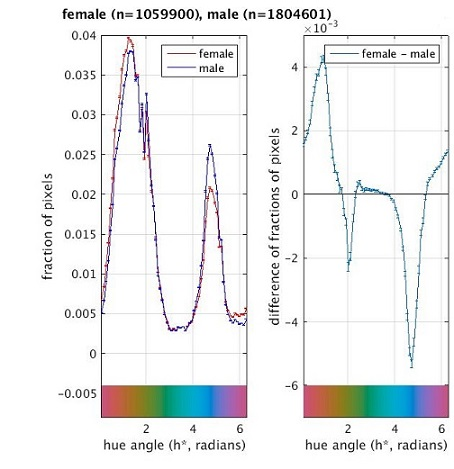
\includegraphics[width=0.489\textwidth]{figures/chapter3/randomhuesmall.jpg}
 \caption{Results on Random dataset. Left: Distribution across hue for male and female photographers. Right: Difference between female and male hue distributions, indicating more reddish hues for women and more bluish hues for men.}
 \label{fig:random}
\end{figure}

\begin{figure*}[th]
\centering
\begin{tabular}{c c}
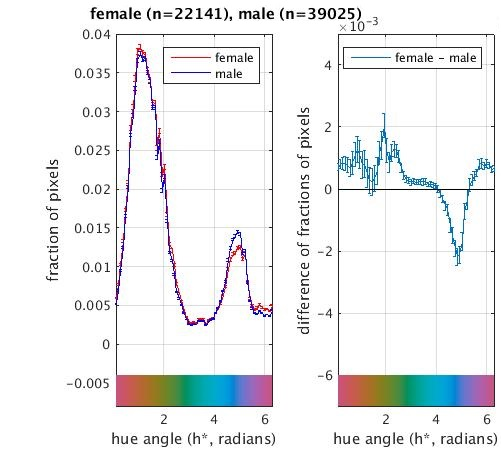
\includegraphics[width=0.45\textwidth]{figures/chapter3/allpeoplehuesmall.jpg} &
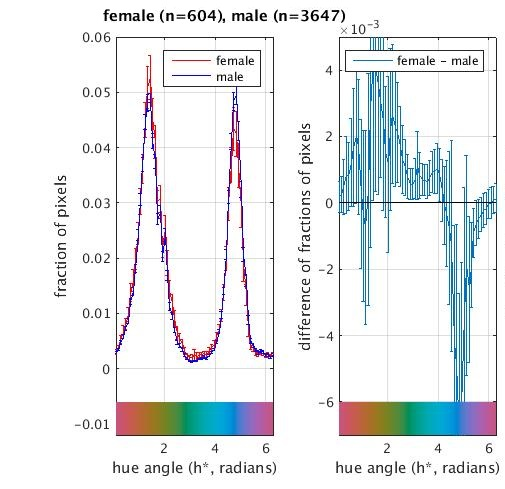
\includegraphics[width=0.45\textwidth]{figures/chapter3/deathvallyhuesmall.jpg} \\
(a) Allpeople dataset&
(b) Death Valley National Park\\
\\
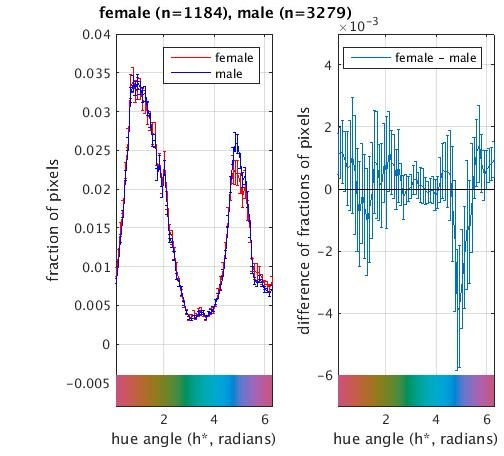
\includegraphics[width=0.45\textwidth]{figures/chapter3/disneyhuesmall.jpg} &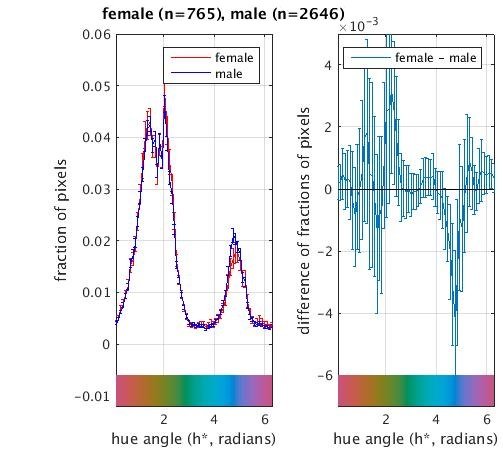
\includegraphics[width=0.45\textwidth]{figures/chapter3/sdzoohuesmall.jpg} \\
(c) Disneyland in Los Angelos&
(d) San Diego Balboa Park\\
\end{tabular}
\caption{Hue distributions and hue difference distributions of 4 different dataset with constraint on content in (a) and locations in (b)-(d).}
\label{fig:allpeople3locations}
\end{figure*}

\begin{figure}[t]
 \centering
    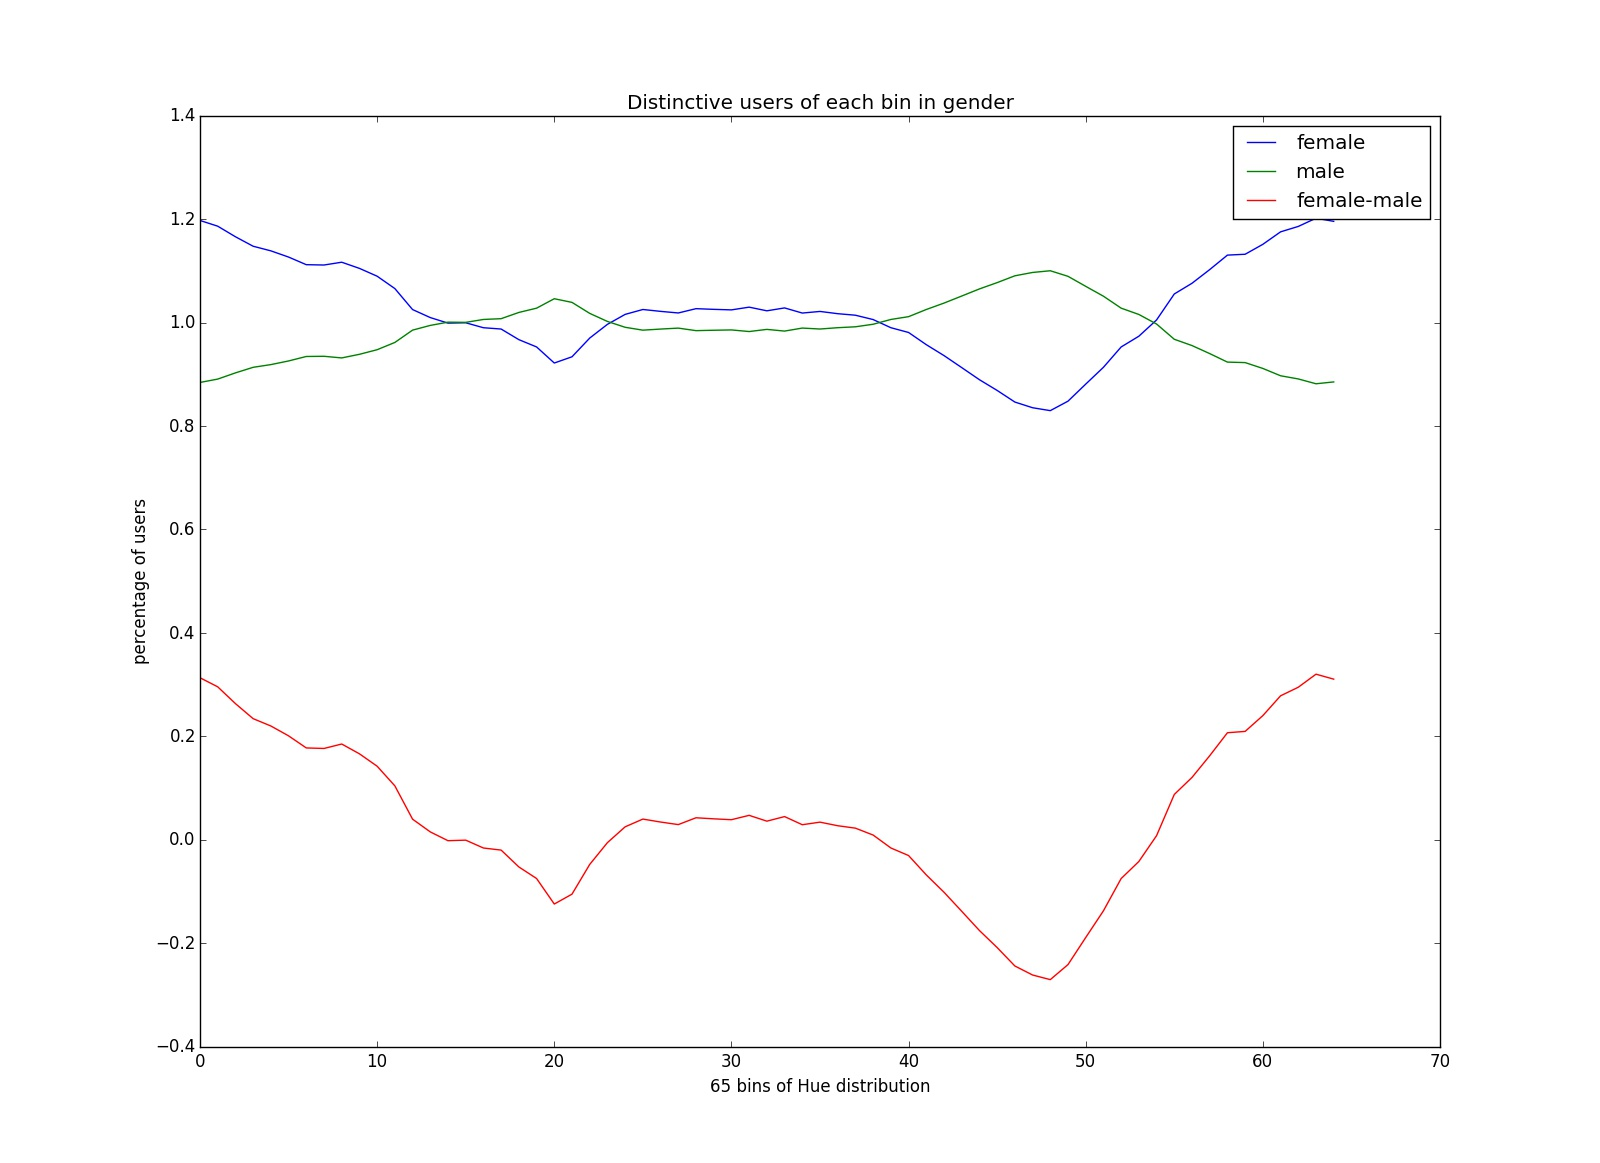
\includegraphics[width=0.489\textwidth]{figures/chapter3/topusergender.jpeg}
 \caption{Number of users with more than $10\%$ color pixels in each color bin (according to Allpeople dataset) showing the consistaent result of gender preference on redish and bluish color.}
 \label{fig:user}
\end{figure}

\section{Genders Preference on Contents}

To give a general idea of what content people take pictures of when they prefer certain colors, we perform a further experiment. Generally people would like to tag their images with the occasion, names of people in the picture and their most interested objects. Therefore, we consider the image tags to represent the content of images.

We rank all the tags appearing in 15 million images in the Random dataset, normalized by users, to find the 500 most frequently used tags. To better visualize the tag distribution, we adopt the hue space of Palmer 32 colors~\cite{palmer32color}. 
These are 32 evenly-speed color points in LCh space, including eight hues in each of two lightness and two chroma values (giving Light, Muted, Dark, and Saturated variants of each hue).

We find images containing more than $10\%$ pixels of each of the 8 hues.
In these images, we aggregate them to users. So each tag used multiple times in images from one user, is only counted once. 
In this way, we compute the tag frequency and entropy across 8 hue centers, for all users, and for male and female users respectively.
We compose the tag distribution maps in two ways.
Firstly, for each hue, find the top 10 most frequently used tags and sort them by the least entropy, presented in Fig. ~\ref{fig:tag} with female user tags on top, male users in the middle and all users at the bottom.
In the second way, the top 500 tags are sorted by entropy value first. Along this list, we find 10 most frequently used tags for each hue. This plot is also presented in Fig. ~\ref{fig:tag} in the same way as the first plot.

\begin{figure*}[th]
\centering
\begin{tabular}{c}
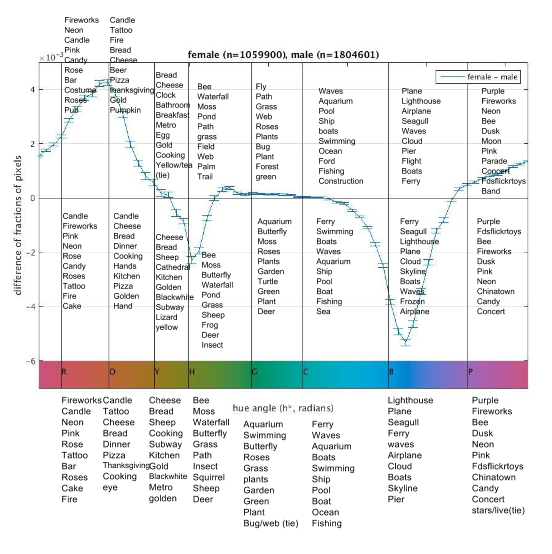
\includegraphics[width=0.65\textwidth]{figures/chapter3/tag1.png} \\
(a) Frequency tag distribution sorted by entropy ascendingly.\\
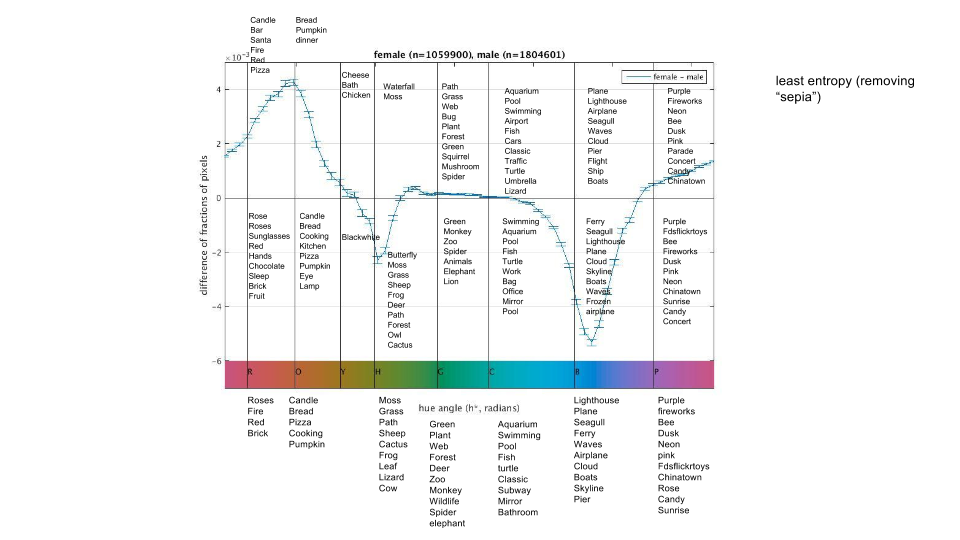
\includegraphics[width=0.65\textwidth]{figures/chapter3/tag2.png} \\
(b) Frequency tag distribution sorted by overall tag entropy.\\
\end{tabular}
\caption{Most concentrated tags on each Palmer color hue for female and male users.}
\label{fig:tag}
\end{figure*}





\section{Color Distribution of Flickr vs. Street View}
The next research question we address is the difference between Flickr photos and the environment where the photographers could have taken pictures. 
We plot the color distribution in histogram of Palmer 32 colors.

To estimate color distributions in the environment, we collect data from Google Street View.
For each geotagged Flickr photo, we query the Google Street View Image API with its GPS information, and download Street View images in 4 view angles (0, 90, 180, 270 degree). If there are no Street View images available for a GPS location, we discard the corresponding Flickr photo.

The result turns out to be very interesting in respect to locations. In Fig. ~\ref{fig:street}, we present the results of three locations of Death Valley National Park, Disneyland at Los Angeles and San Diego Balboa Park. 
In general, we observe the preference of saturated color and reddish color of human compared to the environment.

\begin{figure*}
\centering
\begin{tabular}{m{0.6\linewidth}}
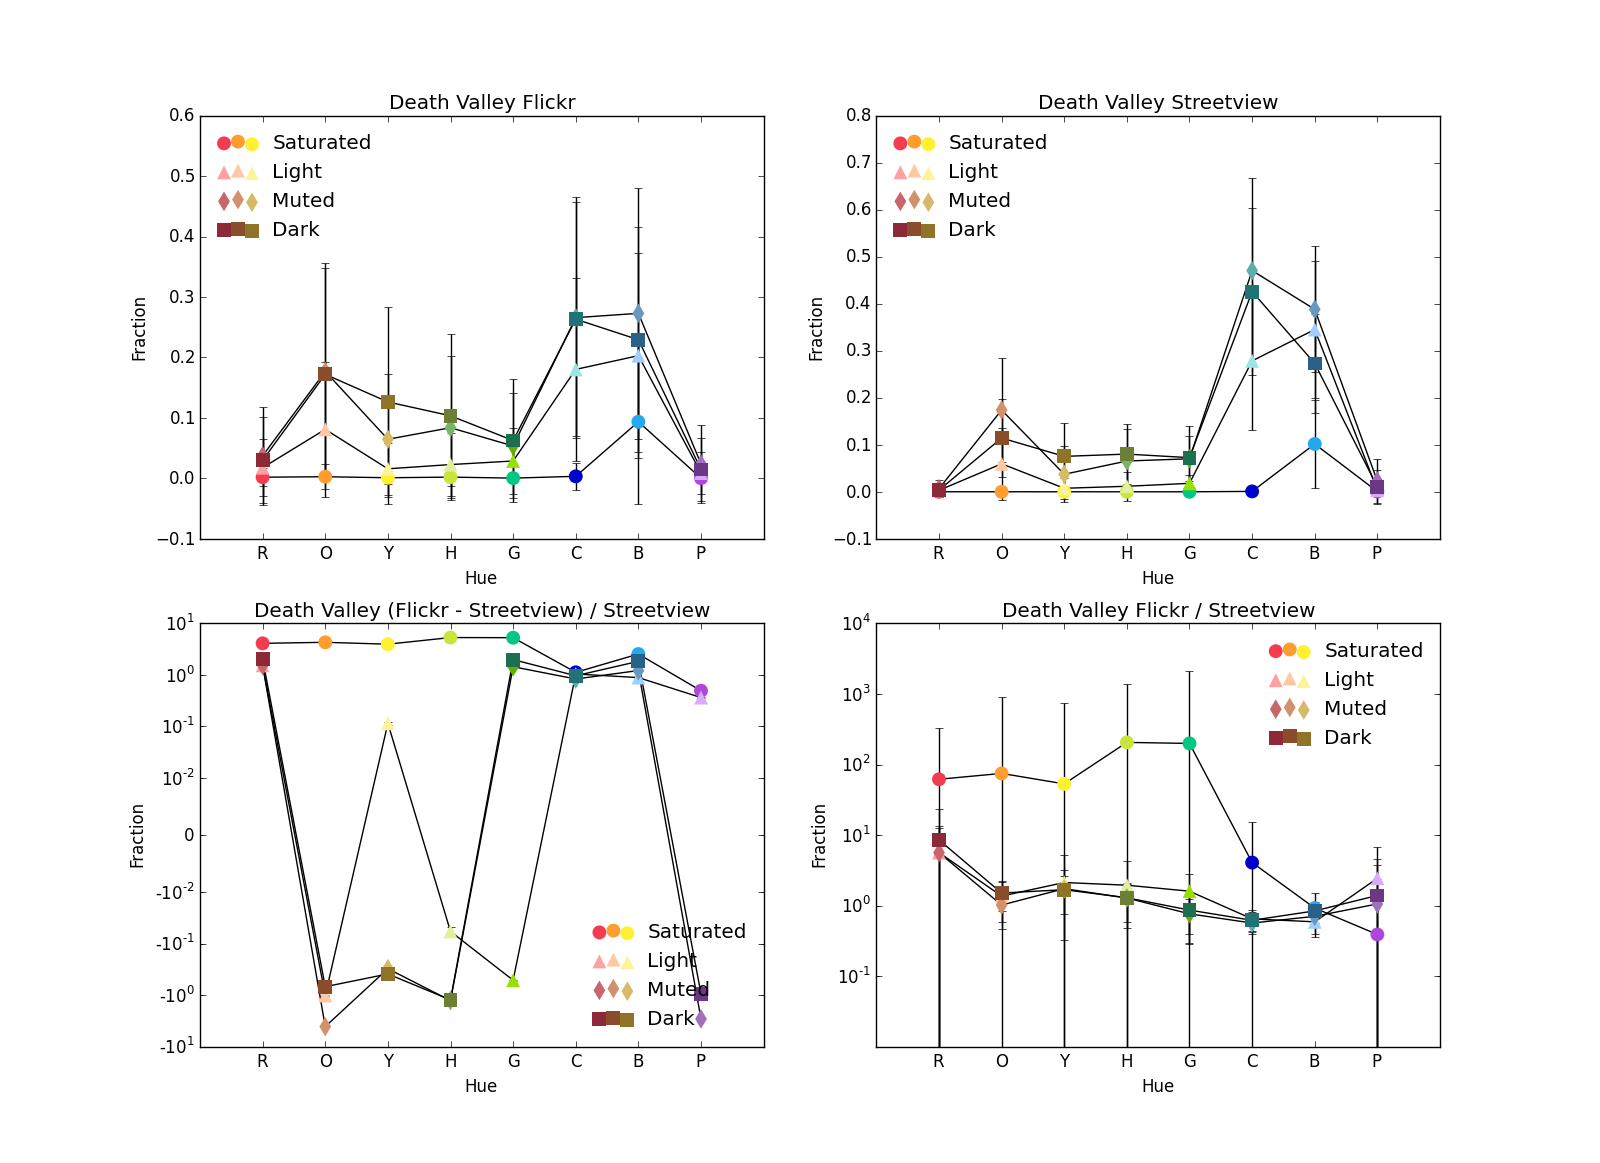
\includegraphics[width=0.55\textwidth]{figures/chapter3/deathvalleyflkstr.png} \\
(a) Deathvalley National Park. It shows photographers prefer warm color in general.\\
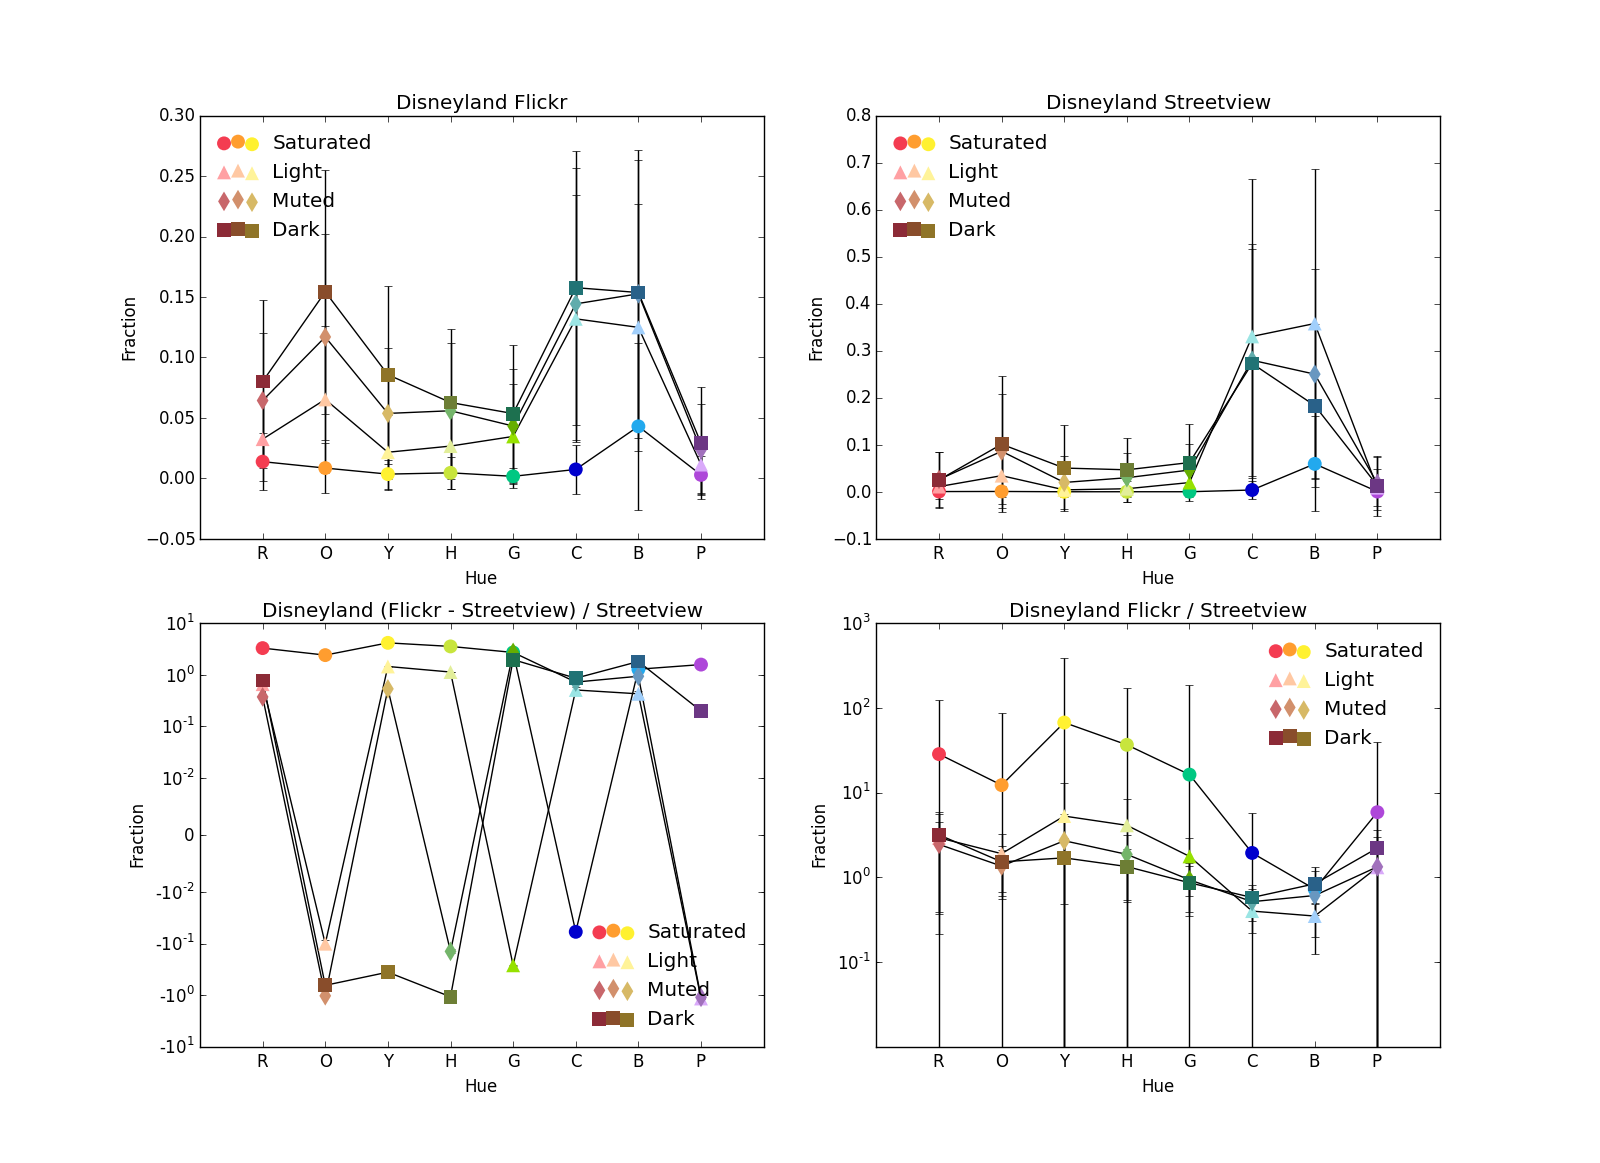
\includegraphics[width=0.55\textwidth]{figures/chapter3/disneyflkstr.png} \\
(b) DisneyLand at Los Angeles. There is more warm color and more saturated color to see in Disneyland so that we see a clearer preference of the photographers.\\
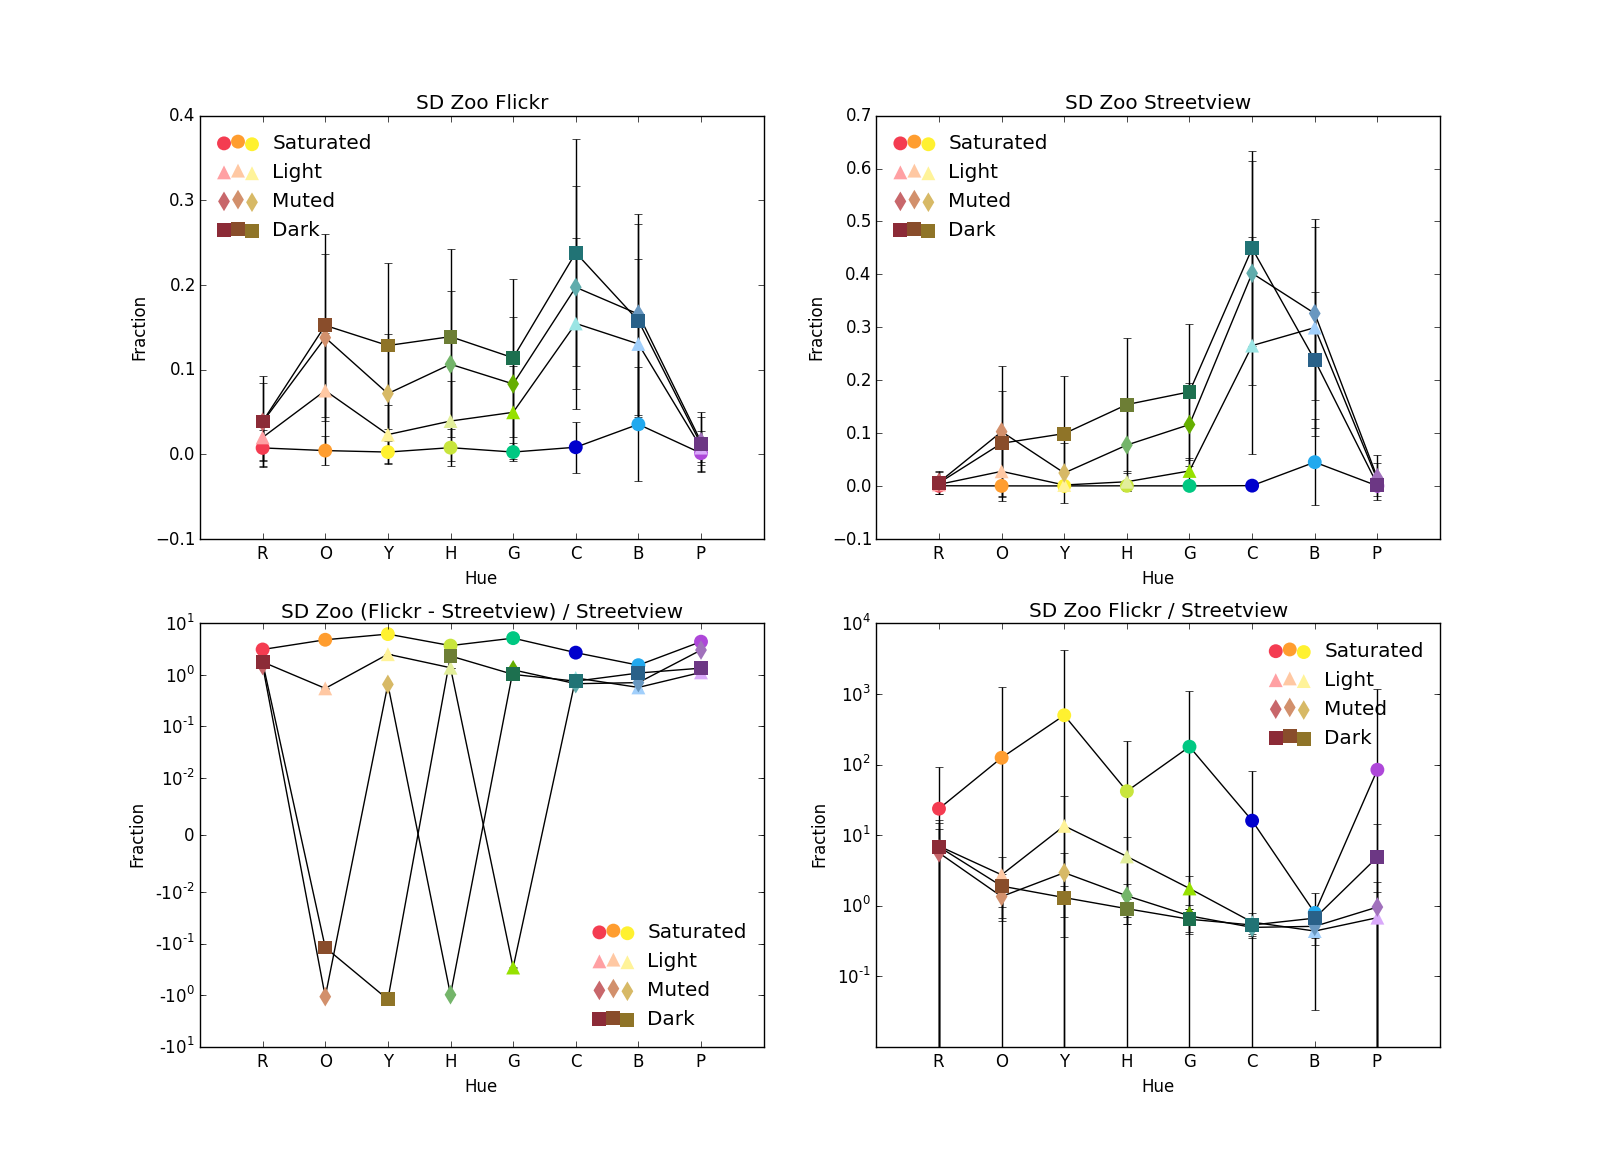
\includegraphics[width=0.55\textwidth]{figures/chapter3/sdzooflkstr.png} \\
(c) San Diego Balboa Park. In this very green place, we observe that people do not show as much interest in greenish objects.\\
\end{tabular}
\caption{Comparison of hue distribution in Palmer's 32 colors for flickr photos and the Google Street View images at the same GPS lcoation.}
\label{fig:street}
\end{figure*}



% \chapter{Detecting Hands based on Visual Appearance}
% Bla Bla Bla
% 
% \chapter{Using Hands to Infer Social Activities}
% Bla Bla Bla
% 
% \chapter{Conclusion}
% \input{conclusion}
% 
% \chapter{Dissertation Timeline}
% \input{timeline}
% 
% \chapter*{Curriculum Vitae}
% \input{cv}


\bibliographystyle{plain}
\bibliography{proposal}

%\include{CV}
\end{document}
